% 原文 printed pp.171--178 / PDF pp.185--192
\providecommand{\chfiveeq}[1]{\par\begin{center}\includegraphics[width=.84\linewidth]{figures/ch05_eq_#1.pdf}\end{center}\par}
\sectionlink{スピンと振動子の世界：デコヒーレンスの標準模型}
% 原文 p.171
\hypertarget{srcpage:171}{}\label{srcpage:171}
いうまでもなく、自然界にはデコヒーレンスが重要な役割を果たす物理系が、無数に存在する。したがって、その一つひとつの系のデコヒーレンスを模型化する作業は、かなり気の遠くなるものに思えるだろう。異なる物理系に出会うたびに、適切な系と環境の模型を作り、その運動を決める作業を、一からやり直す必要があるように見える。中間的・巨視的な尺度で典型的に出会う多体系や相互作用の複雑さを考えれば、どうすれば、この模型化を成し遂げられるだろうか。

幸い、非常に便利な簡単化が助けになる。実用上関心のある多くの状況、ことによると大部分の状況では、環境と相互作用する中心系を、ごく少数の標準模型に写像できることがわかる。このような模型では、中心系を、連続的な位相空間座標で記述され、あるポテンシャル（例えば調和振動子ポテンシャル）の中を運動する粒子として表すか、あるいは系の状態空間が離散的で、実効的に二次元である場合には、スピン$1/2$粒子として表す。同様に、環境は調和振動子またはスピン粒子の集まりとして模型化する。したがって、環境を調和振動子で表すデコヒーレンス模型は、一般に振動子環境模型と呼ばれ、スピン粒子の環境に基づく模型は、スピン環境模型と呼ばれる。用語について一言付け加えると、以下では「熱浴」、または略して「浴」という表現は、熱平衡にある環境を指す。

このような系と環境の表現の選択には、四つの異なる組合せがあるため、デコヒーレンスの主要な標準模型は、合計四つとなる。標準模型は非常に一般的なので、デコヒーレンスの研究において、きわめて重要な役割を果たす。特定の物理的環境に接する、与えられた物理系の詳細は、模型を評価する際の特定のパラメータ集合に、大部分がまとめられる。したがって、任意のパラメータに対して一度模型を解けば、対象の物理的状況と一致するようにパラメータを選ぶだけで、自然界のさまざまな系に、かなり容易に適用できる。

% 原文 p.172
\hypertarget{srcpage:172}{}\label{srcpage:172}
各標準模型は、あるパラメータ領域では、その模型に特有のデコヒーレンスの動力学を生じ、別の領域では、他の模型を近似することがある。例えば、系と環境の結合が弱い極限では、スピン環境模型を振動子環境模型へ写像できる\cite{ref199,ref208}（後の5.4.2節参照）。

本章の構成は次のとおりである。5.1節では、物理系を標準模型に写像する基礎となる、物理的動機と仮定を論じる。続く5.2節では、身の回りの日常世界におけるデコヒーレンスと量子から古典への移行の記述に非常に重要な、最初の標準模型を述べる。これは量子Brown運動の模型である。連続的な位相空間座標で表される粒子が、互いに相互作用しない調和振動子の環境に結合している状況を記述する。

5.3節では、中心系を実効的な二準位系に置き換える。ここでは、中心スピン系が調和振動子のボソン環境と相互作用するため、得られる模型はいわゆるスピン・ボソン模型として知られるようになった。この模型の簡単化した形を解析的に解き、一般的な模型に対するBorn--Markovマスター方程式も導く。

5.4節では、スピン環境模型へ進む。後で論じるように、これらの模型は、超伝導系で見られるような非常に低い温度で、特に重要になる。ここでは、物理的に最も重要な、中心の二準位系（スピン$1/2$粒子で表す）が他のスピンの環境と相互作用する場合に注目する。スピン環境から振動子環境への写像も述べる。

異なるデコヒーレンス模型と、具体的な物理的状況への適用に関する文献は、いまやあまりに膨大で、この分野の全体を捉えようと試みることさえ望み薄である。それでも、本章は主要なデコヒーレンス模型とその物理的重要性について、よい概観を与え、これらの模型を解く際に用いる標準的な手法の一部を示す。どうしても議論は、時に多少技術的になるので、読者は本文をどの程度詳しく学ぶか、好みに応じて選んでよい。最初は標準模型の一つだけに注目し、後で他の模型に戻りたい読者には、5.2節で述べる量子Brown運動の模型から始めることを勧める。この模型はデコヒーレンス研究で決定的に重要なだけでなく、デコヒーレンスの物理的・形式的・概念的に重要な多くの側面を論じる機会も与える。Born--Markovマスター方程式の形式が実際に働く様子を見て、得られたマスター方程式の各項の物理的意味を解析し、スペクトル密度の役割と性質を述べ、デコヒーレンスの動力学と、位相空間における優先状態の環境誘起超選択を示し、このようなデコヒーレンス模型の一般的な限界を論じる。

% 原文 p.173
\hypertarget{srcpage:173}{}\label{srcpage:173}
\subsectionlink{標準模型への写像}
まず、中心系（5.1.1節）と環境（5.1.2節）を調和振動子またはスピン$1/2$粒子に写像する背後にある、物理的な考え方をいくつか述べよう。

\subsubsectionlink{中心系の写像}
多くの場合、系の運動の微視的構造全体ははるかに複雑でも、中心系の関係する運動は、一つか二つの対象座標で記述できる。この座標は連続的でも離散的でもよい。

連続座標の場合、物理的に関心のある典型的な状況は、位相空間座標$\hat X$（位置）、$\hat P$（運動量）で記述され、あるポテンシャル$V(\hat X)$の中を運動する質点である。デコヒーレンスの研究では、原子やイオンなどの粒子が、例えば結晶格子や磁場の「トラップ」に閉じ込められた運動を表す、調和振動子ポテンシャル$V(\hat X)=M\Omega^2\hat X^2/2$を、しばしば考える。自由粒子の場合$V(\hat X)=0$も、量子から古典への移行に明らかに関係する。

位置と運動量が、関係する「古典的」座標として選ばれることは、環境との相互作用、すなわち環境誘起超選択（2.8節参照）の帰結である。量子Brown運動（5.2節）など、多くの重要な場合、中心系の発展は、系の自己Hamiltonian $\hat H_{\mathrm S}$と、系と環境の相互作用Hamiltonian $\hat H_{\mathrm{int}}$に、ほぼ同じ強さで支配される。自然界の相互作用の大部分は、相互作用する両者の距離に依存するため、$\hat H_{\mathrm{int}}$は通常、位置について対角的となる（2.8.4節も参照）。一方、$\hat H_{\mathrm S}$の運動エネルギー項$M\hat P^2/2$は、運動量について対角的である。5.2.5節で論じるように、系の指針状態は、位置空間での完全な局在化と、運動量空間での完全な局在化の妥協として出現し、位相空間でほぼ局在した状態となる\cite{ref086,ref106,ref109}。

離散座標を含む物理的に最も重要な状況は、実効的に二準位系として働く中心系である。これは通常、系が障壁で隔てられた二つのエネルギー極小をもち、そのエネルギーが十分低い（極小のエネルギーに近く、障壁の高さよりはるかに低い）場合に起こる。このとき系の運動は、実効的に二重井戸ポテンシャルに閉じ込められた粒子の運動になる（図5.1）。多くの物理的状況では、各井戸に基底状態以外の励起状態は、存在しても一つか二つしかなく、通常それらは占有されない。こうして、二つの状態が、それぞれ「左」と「右」の井戸への局在に対応する、実効的な二状態系が得られる。さらにこの二つの準位は、スピン$1/2$粒子の二つの量子状態$|0\rangle$（「上向きスピン」）と$|1\rangle$（「下向きスピン」）へ写像できる。

% 原文 p.174
\hypertarget{srcpage:174}{}\label{srcpage:174}
\begin{figure}[htbp]\centering
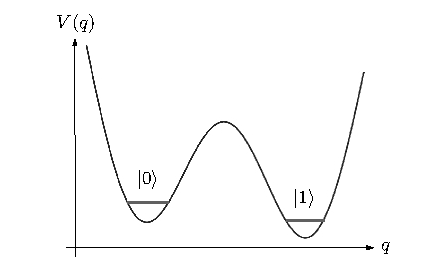
\includegraphics[width=.6\linewidth]{figures/ch05_fig01.pdf}
\caption{二状態系への写像。広がりをもつ座標$q$で記述され、二重井戸ポテンシャル$V(q)$の中を運動する系を考える。多くの場合、系は各井戸の最も低い状態だけを占有し、したがって、左と右の井戸への局在にそれぞれ対応する二つの基底状態$|0\rangle$、$|1\rangle$によって実効的に記述できる。}\label{fig:5.1}
\end{figure}
このような二準位系は量子計算において特に重要であり、量子情報を符号化する量子ビットの物理的実現となる（第7章参照）。

二準位系に固有の運動は、井戸の間の量子トンネル効果から生じ、二つの状態$|0\rangle$と$|1\rangle$の間の遷移をもたらす。状態$|0\rangle$、$|1\rangle$をPauliの$z$スピン演算子$\hat\sigma_z$の固有状態とすれば、トンネル効果は、系のHamiltonianに含まれる
\begin{equation}
\hat H_{\mathrm S}^{\mathrm{tunnel}}=-\frac12\Delta_0(|0\rangle\langle1|+|1\rangle\langle0|)\equiv-\frac12\Delta_0\hat\sigma_x
\tag{5.1}
\end{equation}
という形の項によって媒介される。$\Delta_0$は、いわゆるトンネル行列要素である。二つの井戸の基底状態間のエネルギー差（いわゆる「非対称エネルギー」）は、しばしば、各井戸内の状態のエネルギー間隔と比べて小さく、したがって各井戸の低いエネルギー準位は、ほぼ同じ高さに並ぶ。これにより、一方の井戸、例えば状態$|0\rangle$に対応する左の井戸に局在していた「粒子」が障壁をトンネルしても、通常、右の井戸の励起準位$|1'\rangle\ne|1\rangle$には到達できないことが保証される\cite{ref209}。

\subsubsectionlink{環境の写像}
次に、環境の写像へ移ろう。先に述べたように、ここで関心のある状況は二つある。環境を調和振動子の集まりとして記述する場合と、量子二準位系を表すスピン$1/2$粒子の集まりとして記述する場合である。

% 原文 p.175
\hypertarget{srcpage:175}{}\label{srcpage:175}
\subsubsectionlink*{振動子環境}
多数の調和振動子による環境の表現には、量子電磁力学やスピン波・電子気体模型にさかのぼる長い歴史がある（概観は文献\cite{ref210}参照）。振動子環境は、非局在化したボソン場のモードの準連続体に対応し、中心系のコヒーレンスとエネルギーは、この広がったボソン環境へ、実効的に不可逆に失われていく。「非局在化したモード」とは、個々の調和振動子、すなわち各ボソン場モードの波動関数が、広い空間領域に広がっていることを意味する。この環境モードの非局在性は、調和振動子環境に特有の性質である。

振動子環境は、主としてその一般性の高さのため、デコヒーレンス過程の模型化において、きわめて重要な役割を果たす。十分低いエネルギーでは、相互作用する系と環境の組合せの広いクラスを、調和振動子の環境へ線形に結合した、一つか二つの系の座標で実効的に表せることが示せる。実際、FeynmanとVernon\cite{ref211}が最初に示したように（CaldeiraとLeggettの研究\cite{ref212}も参照）、相互作用が十分弱く、2次摂動論が適用できれば、どのような環境との相互作用も、振動子環境へ線形に結合した系に、厳密に写像できる（この写像は後の5.4.2節で詳しく論じる）。

\subsubsectionlink*{スピン環境}
低温の状況では、通常、スピン環境が適切な模型となる。もちろん、こうした低温は、身の回りの日常世界で通常見られるものではない。しかし実験室では日常的に達成され、多くの実験に不可欠である。特に、巨視的な量子コヒーレンスとデコヒーレンスの研究を目指す実験（第6章参照）、中でも超伝導系を用いるもの（6.3節）を動作させるには、絶対零度に近い温度が必要となる。これらの実験は、量子計算機の実装に用いる量子ビット系の実現という点でも、大きな関心の対象である（第7章）。

したがって、低温領域のデコヒーレンスを正しく模型化することは非常に重要である。実験的証拠によれば、この領域のデコヒーレンスは、通常、常磁性スピン、常磁性電子不純物、トンネルする電荷、欠陥、核スピンなど、局在したモードとの相互作用に支配される\cite{ref199,ref200,ref213}（6.3節、6.4.2節も参照）。これらのモードが局在しているとは、振動子環境とは対照的に、各モードに付随する波動関数が、空間の小さな領域に閉じ込められていることを意味する。

% 原文 p.176
\hypertarget{srcpage:176}{}\label{srcpage:176}
各局在モードは、有限のエネルギーカットオフをもつ有限次元Hilbert空間で記述される。したがって、これらのモードを離散状態の集合として模型化し、スピン系へ写像できる。大部分の関心ある場合には、関係する状態は二つだけなので、局在モードの環境をスピン$1/2$粒子の環境へ写像できる。スピン環境のモードは、対象となる物理系自体の一部（「内部環境」を構成する）でも、周囲の基板の一部でもよい。例えば、いわゆる超伝導量子干渉素子（SQUID。詳細は6.3節参照）では、磁束座標は、SQUIDのバルク物質を構成し、磁束の侵入長内にある膨大な核スピンの集まりだけでなく、物質内のあらゆる不純物にも、電磁気的に結合する\cite{ref214}。

スピン環境が、重要で、しばしば支配的なデコヒーレンス源であることを示す例は、ほかにも数多い。巨視的尺度のコヒーレントな重ね合わせ状態を作ろうとするとき、研究者は、熱的環境を「凍結」させてデコヒーレンス効果を最小にするため、通常、非常に低い温度で実験を行う。この熱的環境こそ、先に述べた非局在化したボソンモード、すなわち調和振動子の浴である。しかし、SQUIDなどの超伝導系でしばしば行うように、温度を絶対零度の近傍まで下げても、物質内に本来存在する核スピンや不純物などの局在モードの影響は、通常変わらない。そのため、これらのデコヒーレンス源が、この低温領域で支配的になる。

\subsubsectionlink*{振動子環境とスピン環境：相違点と類似点}
振動子環境とスピン環境を用いる物理的動機を別々に概説したので、次に、両者の重要な相違点と類似点を論じ、説明をまとめよう。

先に述べたように、弱結合極限では振動子環境は普遍的な環境となる。任意の環境と系の相互作用を、同等な振動子環境への線形結合へ写像できる\cite{ref211,ref212}。この意味で、線形に結合した振動子環境は、弱結合極限の妥当性を前提としているともいえる。さらに、各モードの結合強度は、通常、環境の振動子数$N$に対して$\propto1/\sqrt N$とスケールすると仮定する。このスケーリングにより、すべてのモードの寄与を足し合わせた値は$N$に依存しなくなり、したがって熱力学的極限$N\longrightarrow\infty$が明確に定義される。

結合が弱く、$N$に依存するという、この組合せの仮定は、中心系は一般に環境の振動子の集団的影響を強く受ける一方、環境の個々の振動子は、系との結合から無視できるほど小さな影響しか受けないことを意味する。

% 原文 p.177
\hypertarget{srcpage:177}{}\label{srcpage:177}
中心系が環境に及ぼした効果は、通常非常に速く減衰する（これは4.2節で導入したBorn--Markov近似に対応する）。したがって、環境自身の運動は、中心系の運動からほとんど影響を受けない。

しばしば強調されるように\cite{ref199,ref200,ref210,ref215,ref216}、弱く、$N$に依存する結合という仮定は、スピン環境で表す局在モードの場合、通常は物理的に妥当でない。多くの物理的に興味ある状況で、個々の環境スピンと、通常は巨視的な中心系の座標との結合の強さに付随するエネルギー尺度は、Hamiltonianの残りの項で定まる他のエネルギー尺度に優越する。特に、環境のスピン間相互作用は、通常極端に弱い。異なる環境モードの波動関数が局在し、空間的な重なりがわずかしかないためである。環境スピンは、位相空間が制限されているため、他の外部の非局在モードにも、通常非常に弱くしか結合しない。さらに、スピン環境の場合、振動子環境のように結合を$N$に強く依存させてスケールすることは、通常、必要でも物理的に妥当でもないと論じられている\cite{ref199,ref200}（ただし文献では、$\propto1/N$などのスピン結合のスケーリングが、時に仮定されている。例えば文献\cite{ref217}参照）。

したがって、スピン環境で関心があるのは、環境のスピン数に依存しない、またはごく弱くしか依存しない結合係数で記述される強結合領域である。これにより、環境、ひいてはそれに結合する系は、振動子環境の場合と非常に異なる振る舞いを示す。通常、スピン環境のモードは、中心系を記述する関係座標に非常に強く「従属」するようになり、したがって環境の運動は中心スピンの運動から大きな影響を受ける\cite{ref199}。

この振る舞いは、環境内の固有の揺らぎ、すなわち自己Hamiltonianとスピン間相互作用による運動が凍結する零温度極限においてさえ、環境の動的変化を可能にする。この効果の帰結の一つとして、先に述べたように、絶対零度に近い温度、例えば$\mu\mathrm K$でも、スピン環境は通常、系に顕著なデコヒーレンス作用を及ぼす。一方、振動子浴のデコヒーレンス効果は、そのような温度では大部分の場合、比較して無視できるほど小さくなる。したがって、零度近くで比較的速いデコヒーレンス率を実験で観測したなら、局在モードとの相互作用が主要なデコヒーレンス源であることが示唆される。これにより、非局在化したボソン場モードと、局在したスピン型モードという、二つのデコヒーレンス源を、実験的に区別できる。
